\documentclass[../dejiny-rodu-prusiku.tex]{subfiles}

\begin{document}

% str 20 @ 29
\chapter{Větev Výrov}

\section{Zakladatel Vojtěch Prusík 1777 - 1841}
Vesnice Výrov leží západně od města Kralovic a v době, kdy píšeme tyto dějiny rodu má asi 500 obyva­tel. Sedlec, odkud celý náš rod původně vzešel, má sice dnes asi jen 130 obyvatel, ale je mnohem starší. Vznikl ve XII. století, kdežto obec Výrov byla zalo­žena v roce 1300 a to klášterem plasským z části dvora Sechutic. Tento dvůr má ovšem mnohem starší historii, neboť se připomíná již v roce 1144, kdy kníže Vladislav II. založil klášter plasský. Sechutice byly dvoje, Horní a Dolní. Na pozemcích Dolních Sechutic, kde byl dvůr, byla tedy založena později vesnice Výrov.

Uprostřed vsi je statek číslo 18, kde se od pradávna říkalo "U Boudů".  Léta Páně 1610 v pondělí po sv. Bartoloměji, jak je v zápise Veyrovské rychty, „stala se smlouva celá a dokonalá a trh dobrovolný mezi urozeným pánem Václavem Kohoutem z Lichtenfeldu, úřední­kem panství Kaceřovského s jedné a Pavlem Boudou, rychtářem ve vsi Veyrově, poddaným J. M. páně se strany druhé a to takový, jakož jest J. M. pán témuž panu Václavovi Kohoutovi grunt slove k ř í ž o v s k ý v též vsi darovati ráčil. Takový grunt jest týž pan Václav Kohout je­mu Pavlovi Boudoví za patnáct kop míšeňských prodal“.

Anna Fenclová, která se v tomto gruntě 30. ledna 1785 na­rodila, byla pokrevním potomkem tohoto prvního majitele, Pavla Boudy. Ji si vzal za manželku 8. října 1803 Vojtěch Prusík, zakladatel větve "Výrov". Že se i jeho bratr v ten den se sestrou Anny, Rosalií oženil v mladém věku 17 let a usadil se v Sedlci jako samostatný hospo­dář, vysvětluje se vážnou dobou. Napoleonské války byly v plném proudu a samostatní hospodáři bývali vojny uchráněni.

Statek u Boudů ve Výrově, podle své polohy i výměry polí a luk, býval významnější a z něho bývali určováni rychtáři a později voleni starostové obce. Před vchodem stály mohutné rozložité topoly, jejichž vrcholy, ač stojí stromy v údolí, bylo vidět již od sv. Jana nebo na pěšině od Kralovic. Statek pravděpodobně vznikl ihned při založení obce. Hospodářství mělo asi 35 ha. Když se Vojtěch Prusík přiženil do Výrova, stal se podle zvyku rychtářem. Byl jím asi 35 let. Na rychtě se čepovalo pivo z plasského panského pivovaru a tímto zařízením si vrchnost zajišťovala odbyt. Rychtář Vojtěch Prusík byl v obci velmi oblíben a i když přišel do Výrova v do­bě roboty nebylo mezi jím a osadníky neshod. U gruntu byla také povinná dvojspřežní robota s koňmi po dobu 156 dní a robota pěší 26 dní. Samozřejmě byly další povinné poplatky, panské dávky, desátek kralovickému faráři, kam obec příslušela a jiné povinnosti. Za humny, směrem ke Kopidlu stojí ještě dnes železný kříž, který v roce 1831 postavil Vojtěch Prusík.

% str 21 @ 30
Jako rychtář jezdíval Vojtěch téměř každou sobotu na koni pro instrukce k panu direktorovi do Plas. Tam se scházel s ostatními rychtáři z okolních obcí, získával tím mnoho známostí a podle vyprávění byl všude velmi oblíben. Byl to velký, silný muž a velmi pobožný. On jako i všichni naši předci od roku 1650 a všichni zase po něm byli katolíci. Jedině do proti­reformace byli naši předci jiné víry. Na Kralovicku byla jediná fara katolická v Žebnici a všechny ostat­ní byly osazeny luteránskými pastory. Také v Kralo­vicích, Potvorově a Všesulově podávalo se "pod obojí". Protože Sedlec patřil farností k Potvorovu, nebyli tehdy naši předci také katolíky, počínaje prvním na­ším známým předkem Vojtěchem Prusíkem.

Když se Vojtěch přiženil do Výrova žil ještě jeho tchán Matěj Fencl se svou manželkou Kateřinou. Matěj se narodil v roce 1746 a zemřel na gruntě na výměnku 3. února 1820. Kateřina byla rozená Hubková z Kočína, kde se narodila v roce 1753. Dožila se úctyhodného vě­ku 98 let a do poslední chvíle to byla velmi čilá stařenka. Zvláště milovala svého vnuka Václava Prusíka, který převzal grunt po otci a v jeho náručí také usnula na věky 3. března 1851. Ten den ještě ráno pekla chléb.

Vojtěch a Anna měli spolu osm dětí. Nejstarší ze všech byla Anna. Narodila se 4. ledna 1805. Její otec seznámil se na rychtářských schůzkách v Plasích s mladým vdovcem, rychtářem Jakubem Štěpánkem z Horní Břízy, kde se jeho usedlosti říkalo "U Kubíků". Když bylo Anně 17 let provdala se za Štěpánka 10. září 1822. Dožila se tam 78 let, zemřela 11. března 1883. Je zakladatelkou odnože, kterou nazveme "Horní Bříza I".

Druhým dítětem byla Rosalie. Narodila se 3. září 1807. Patrně vlivem své sestry, usazené již v Horní Bříze, vdala se tam i ona. Vzala si 6. června 1826 sedláka Vojtěcha Kareza z č. 3. Zemřela tam v mladém věku 44 let o pouti dne 9. května 1851. Je zakladatelkou odnože tzv. "Horní Bříza II".

Další dcerou byla Marie. Měla špatný osud. Narodila se 20. května 1815 a ve svých 18 letech se 26. 1istopadu 1833 provdala za sedláka z Výrova č. 6, Josefa Štefla. Ještě dnes v této usedlosti žijí její potomci. Marie Šteflová zemřela krátce po porodu třetího dítěte 27. prosince 1844. Bylo jí pouze 29 let. Založila odnož tzv."Výrov I".

Čtvrtou a poslední dcerou Vojtěcha a Anny byla Veronika. Bylo to jejich nejmladší dítě. Narodila se 20. ledna 1826 a provdala se do malé vesničky, ležící již za řekou Mží, Kostelce nad Mží. Vzala si 20. ledna 1846 sedláka Jana Hořejše a po brzkém ovdovění v r. 1854 se vdala za Jana Folka. Zemřela mladá 7. listopadu 1865. Je zakladatelkou odnože tzv. "Kostelec nad Mží".

% str 21+1 @ 31

\begin{figure}
\centering
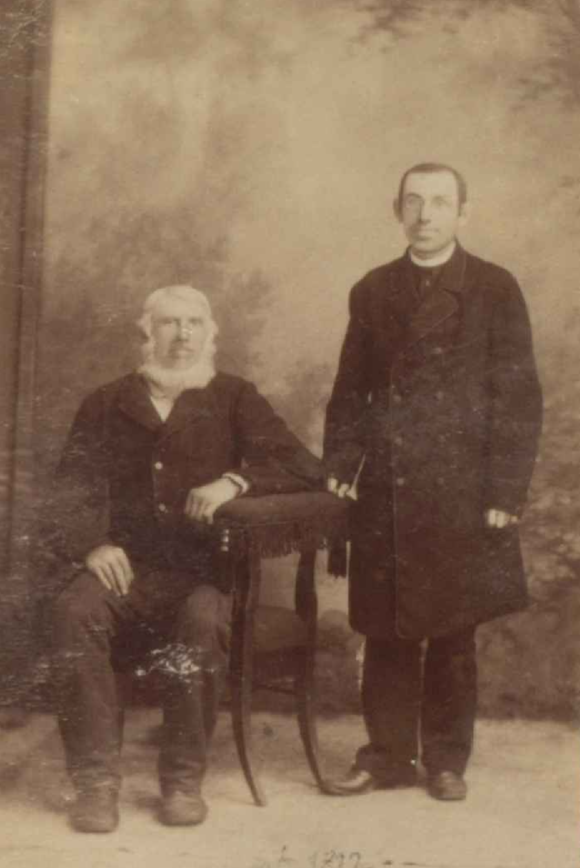
\includegraphics[width=\textwidth, height=\textheight, keepaspectratio]{031-a-tomas_prusik_se_synem}
\caption{Tomáš Prusík se synem knězem Tomášem. Narodil se 1812 ve Výrově a přiženil se 1835 do Horní Břízy. Zakladatel odnože; 1812 - 1897}
\label{fig:031-a-tomas_prusik_se_synem}
\end{figure}

\begin{figure}
\centering
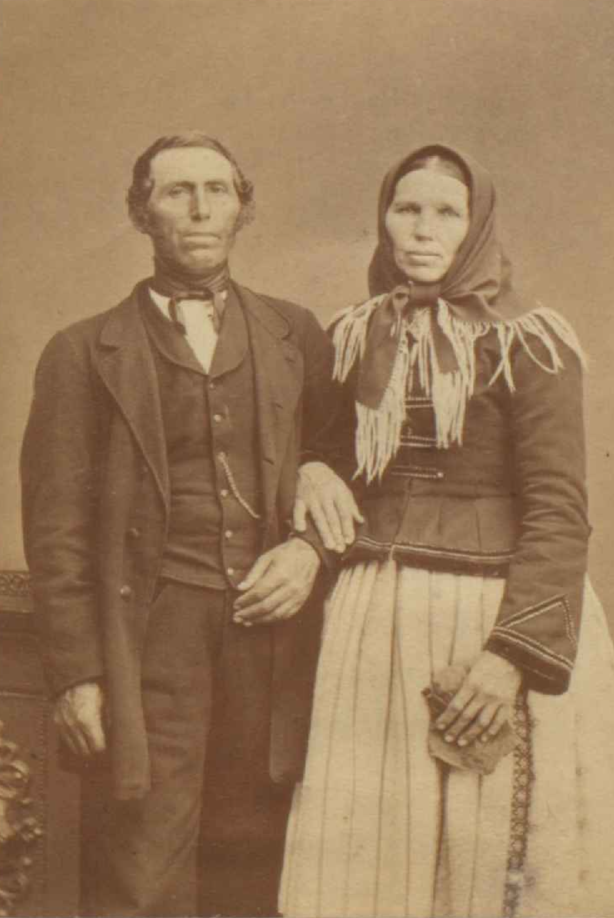
\includegraphics[width=\textwidth, height=\textheight, keepaspectratio]{031-b-vaclav_prusik_se_zenou}
\caption{Václav Prusík se ženou Josefou roz. Kotasovou z Kozojed. Narodil se r. 1822 ve Výrově, kde převzal grunt a stal se zakladatelem silné odnože. 1822 - 1892}
\label{fig:031-b-vaclav_prusik_se_zenou}
\end{figure}

\begin{figure}
\centering
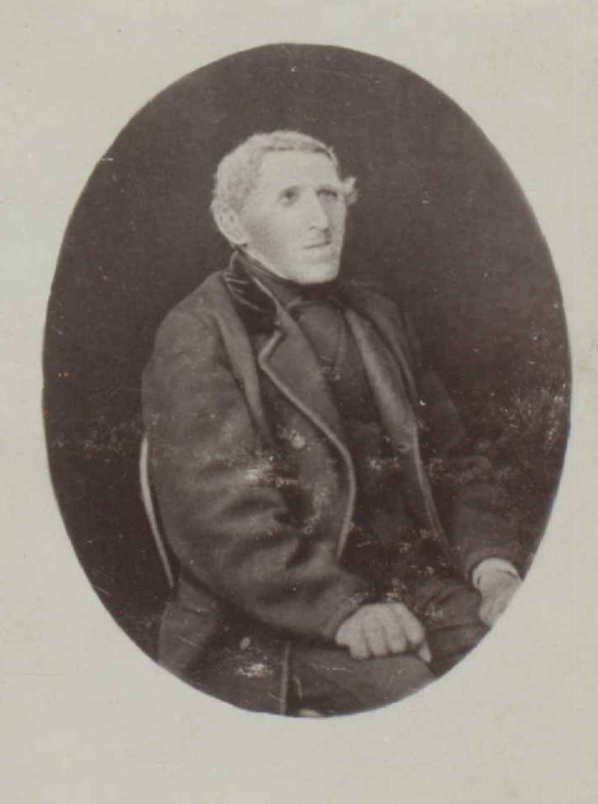
\includegraphics[width=\textwidth, height=\textheight, keepaspectratio]{031-c-matej_prusik}
\caption{Matěj Prusík narozený 1818 ve Výrově, přiženil se r. 1843 do Hodyně, kde založil rodovou odnož. 1818 - 1900}
\label{fig:031-c-matej_prusik}
\end{figure}


% str 22 @ 32
Nejstarším synem byl Blažej Prusík. Narodil se 1. úno­ra 1810 a při křtu v Kralovicích dostal jméno po svém dědovi Blažejovi, který tehdy žil již na výměnku v Sedlci. Blažej Prusík zaujímá zvláštní kapitolu v dějinách našeho rodu. Stal se knězem a opravdovým dobrodincem rodu. O jeho životě budeme podrobně vyprávěti později. Zemřel v Praze 22. srpna 1888.

Dalším synem byl Tomáš. Narodil se 19. listopadu 1812 a přiženil se 24. února 1835 do Horní Břízy, kde tehdy žily již jeho dvě sestry. Jeho ženou byla Kateřina Beránková z gruntu č. 26 tzv. Fakanovského. Tomáš Prusík zemřel tam 19. dubna 1897 a je zakladatelem odnože tzv. "Horní Bříza III".

Třetím synem byl Matěj narozený 22. února 1818. Vzal si za ženu Annu Fakanovou a usadil se v gruntě č. 17 v Hodyni tzv. Lajbovském. Tam zemřel 17. října 1900 a je zakladatelem odnože tzv. "Hodyně".

Čtvrtým synem, nejmladším byl Václav. Narodil se 7. září 1822 a stal se později dědicem gruntu "U Boudů". Za ženu měl Josefu Kotasovou z Kozojed. Měli svatbu 30. led­na 1843. Václav Prusík zemřel 11. února 1892 ve Výrově. Je zakladatelem odnože tzv. "Výrov II“.

Rychtář Vojtěch Prusík nedožil se vysokého věku. Zemřel 1841 14. března na souchotiny /TBC/. Bylo mu 64 let. Jeho žena Anna ho přežila o 18 let a tchyně o 10 let. Anna zemřela 6. ledna 1859. Žila spokojeně na výměnku u svého nejmladšího syna Václava až do smrti.

Vesnice Výrov spolu se Sedlcem, Plasy a Stražištěm sta­la se tedy dalším východiskem početné rodové větve a je proto pro nás tak významná. Nyní budeme Vás seznamovati se všemi potomky a členy této větve a jejich osudy až do nynějších časů.

% str 22+1 @ 33
\begin{figure}
\centering
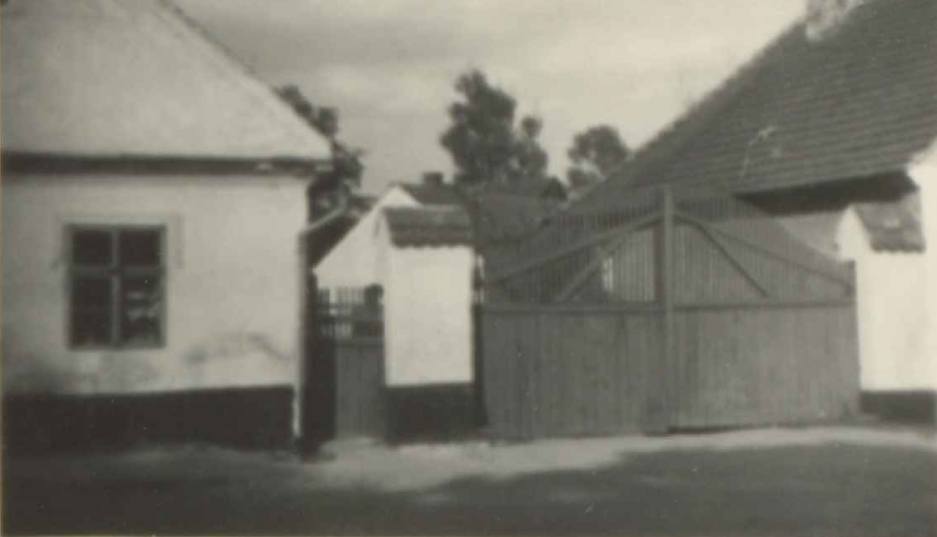
\includegraphics[width=\textwidth, height=\textheight, keepaspectratio]{033-a-statek_v_horni_brize}
\caption{Statek č. 26 v Horní říze, kam se přiženil roku 1835 Tomáš Prusík z Výrova}
\label{fig:033-a-statek_v_horni_brize}
\end{figure}

\begin{figure}
\centering
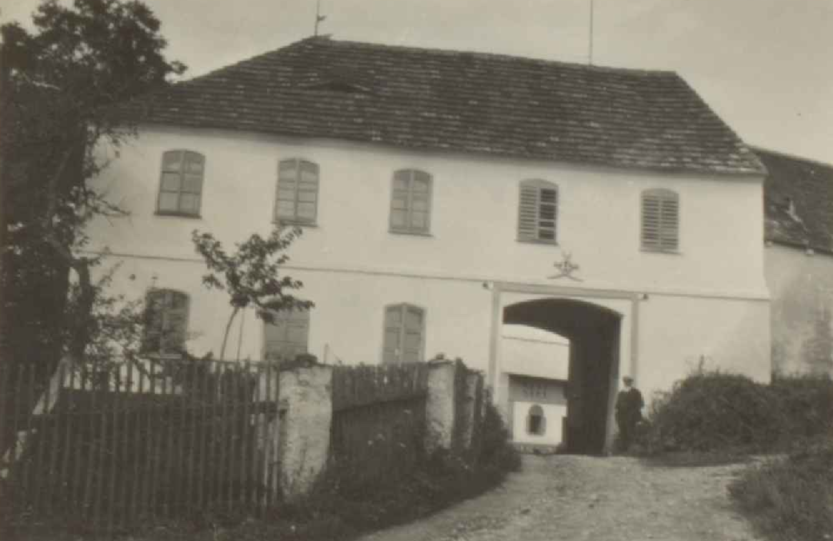
\includegraphics[width=\textwidth, height=\textheight, keepaspectratio]{033-b-statek_prusiku_v_hodyni}
\caption{Statek Prusíků v Hodyni, sídle jedné rodové odnože od roku 1843}
\label{fig:033-b-statek_prusiku_v_hodyni}
\end{figure}

\begin{figure}
\centering
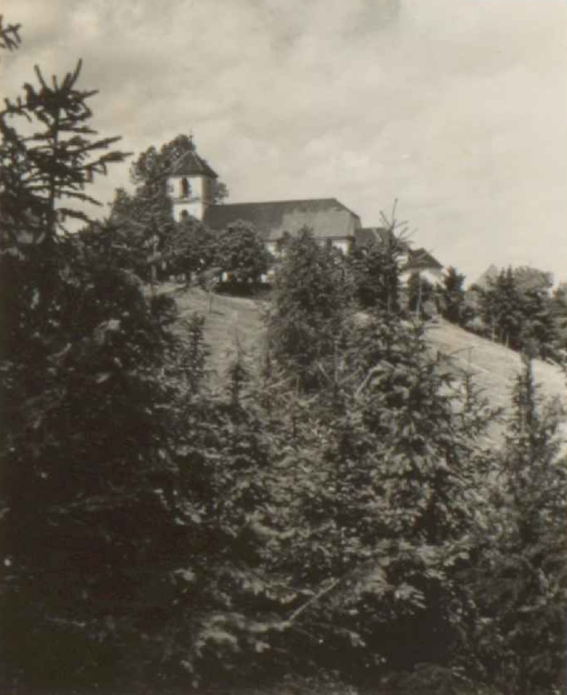
\includegraphics[width=\textwidth, height=\textheight, keepaspectratio]{033-c-kostelec_nad_mzi}
\caption{Kostelec nad Mží, kam se roku 1846 provdala Veronika Prusíková z Výrova}
\label{fig:033-c-kostelec_nad_mzi}
\end{figure}

\begin{figure}
\centering
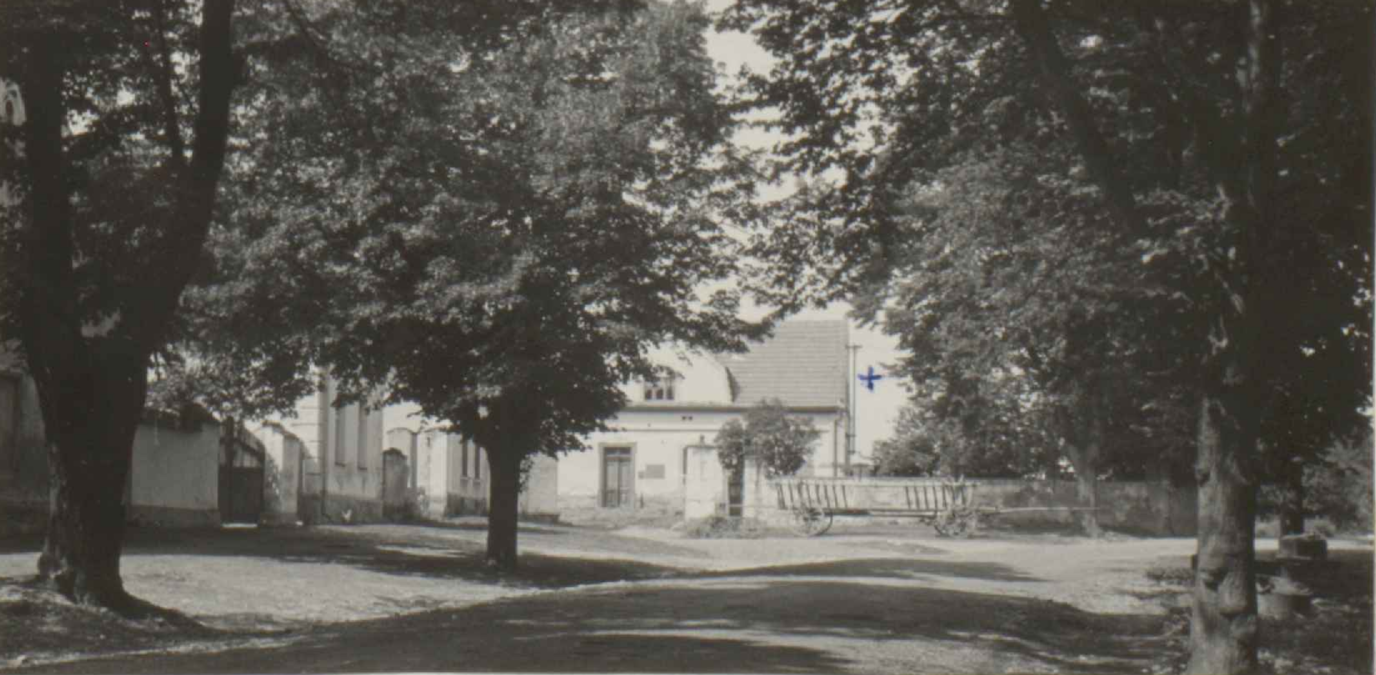
\includegraphics[width=\textwidth, height=\textheight, keepaspectratio]{033-d-statek_kouklu}
\caption{Statek Kouklů (Kymlů) v Bílově, kde byla provdána Kateřina Prusíková ze Sedlce, zakladatelka rodové odnože větve Sedlec}
\label{fig:033-d-statek_kouklu}
\end{figure}

\end{document}
